\chapter{Dynamic Model of the Quadrotor \label{ch:model}}

In this chapter, the derivation of the quadrotor model is provided. This result
is very important because it describes how the helicopter moves according to its
inputs. Thanks to these equations it is possible to define and predict the positions
reached by the helicopter by investigating just the four motor speeds. The model
equations will be ”inverted” in the next chapter (Control algorithms) to identify
which inputs are needed to reach a certain position.
\\\\
The first section (\fullref{sec:configurations}) shows the main idea of the quadrotor
dynamics and describes intuitively which movements are allowed and how it
manages to perform stationary flight (hovering).
\\\\
The second section () provides the model information
with physics and mathematical derivations. In this work, the Newton-Euler
formalism and the Euler angles theories have been chosen.
\\\\
In the third section (\fullref{sec:nonlinear}), additional information was added to
the model taking into account the whole motor system which is composed of the
motor itself, the reduction gears and the propeller.
\\\\
The last section (\fullref{sec:linearized}) provides an overview of the architecture:
connections between devices and abstraction of the software and task.

\section{Quadrotors Configurations}
\label{sec:configurations}
As the term `quadrotor' refers to a multirotor whose thrust is generated from four motors and propellers, quadrotors can be built in multiple ways as long as they comply with the established definition. There are some configurations that are already standardized being widely used by commercial manufacturers and hobbyists, such as the `+' and `X' configurations.
%\\\\
%\url{https://www.google.com/search?q=why+\%2B+or+x+configuration+quadcopter&ie=utf-8&oe=utf-8&client=firefox-b-ab&gfe_rd=cr&dcr=0&ei=Mr0BWrW9HtHk8AfXm7fADQ}
%\\\\
%\url{https://community.micro-motor-warehouse.com/t/vs-x-configuration/2673}
%\\\\
%\url{https://www.quora.com/Why-is-x-configuration-preferred-over-+-config-of-quadcopter}
%\\\\
%\url{https://www.rcgroups.com/forums/showthread.php?1203569-Quad-X-vs-configuration}


\subsection{`+' Configuration}
The geometry used in quadrotors built in `+' configuration is shown in Fig. \ref{fig:quadcopterplus}.
\\
\begin{figure}[H]
\begin{center}
  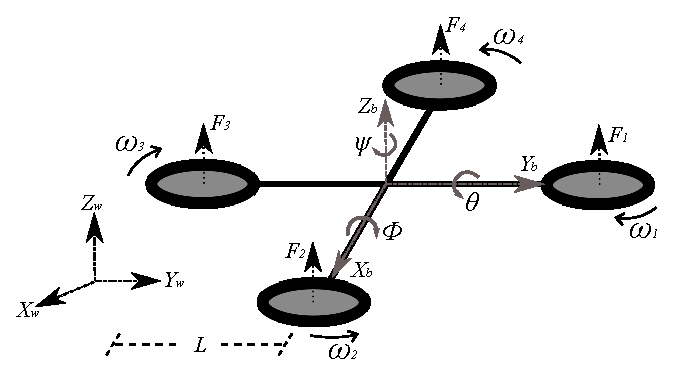
\includegraphics[width=0.90\textwidth]{quadcopterplus.eps}
\caption{Quadrotor geometry in `+' configuration} 
    \label{fig:quadcopterplus}
    \end{center}
\end{figure}
Where, ($\phi$, $\theta$, $\psi$) are the angular deviations (pitch, roll and yaw, respectively) of the quadrotor about the body-frame,
 ($x$, $y$, $z$) are the body-frame axes,  ($X_W$, $Y_W$, $Z_W$) are the earth-frame axes, $L$ is the distance from the quadrotor center of gravity ($CoG$) to the motor center, $F_{M_i}$ is the thrust force exerted by each motor, and $\omega_i$ is the angular velocity of each motor, with $i = 1,2,3,4$. 
\\\\
In this configuration, the body-frame axes $x$ and $y$, coincide with the lines that connect motors of opposite sides in the quadrotor frame. This means that, in order to change the pitch or roll angles, only the angular velocities $\omega_i$ of two motors must be modified, ($\omega_1$, $\omega_3$) for pitch,  and ($\omega_2$, $\omega_4$) for roll, while the generated torques for roll and pitch are applied at a distance of $L$ from the quadrotor $CoG$. Here, $M_1$ is considered as the front motor, $M_3$ as the rear one, $M_2$ as the right motor, and $M_4$ as the left motor. 
\\\\
Even though the quadrotor has 6 DOF, it is equipped just with four propellers, hence it is not possible to reach a desired set-point for all the DOF, but at maximum four. However, thanks to its structure, it is quite easy to chose the four best controllable variables and to decouple them to make the controller easier. The four quadrotor targets are thus related to the four basic movements which allow the helicopter to reach a certain height and attitude. It follows the description of these basic movements.


\subsubsection{Throttle $u$ [$N$]}
\begin{equation}
u = \sum_{i=1}^{4}F_{M_i}
\end{equation}

\subsubsection{Yaw Torque $\tau_{\psi}$ [$N\cdot m$]}
As can be seen in Fig. \ref{fig:quadcopterplus}, $M_1$ and $M_3$ have a clockwise rotation while $M_2$ and $M_4$ rotate counter-clockwise. This configuration of opposite pairs rotational directions allows the system to control its conservation of momentum and thus change its yaw angle in a controlled manner without the need of a tail rotor used in the standard helicopter structure (\cite{Bresciani2008}). In `+' configuration, the fact that the pitch and roll angles are controlled using only two motors that rotate in the same direction, leads to large changes in the thrust force of the other two motors to achieve momentum conservation.
\begin{equation}
\tau_{\psi} = K_{m}(F_{M_2} + F_{M_4} - F_{M_1} - F_{M_3})
\end{equation}

\subsubsection{Roll Torque $\tau_{\theta}$ [$N\cdot m$]}
\begin{equation}
\tau_{\theta} = L(F_{M_4}-F_{M_2})
\end{equation}

\subsubsection{Pitch Torque $\tau_{\phi}$ [$N\cdot m$]}
\begin{equation}
\tau_{\phi} = L(F_{M_3}-F_{M_1})
\end{equation}

\subsubsection{Inputs Setting in `+' Configuration}
\begin{equation}
	U = \begin{bmatrix}
	u\\[5pt]
	\tau_{\psi}\\[5pt]
	\tau_{\theta}\\[5pt]
	\tau_{\phi}
	\end{bmatrix} = \begin{bmatrix}
	1 & 1 & 1 & 1 \\[5pt]
	-K_{m} & K_{m} & -K_{m} & K_{m}\\[5pt]
	0 & -L & 0 & L\\[5pt]
	-L & 0 & L & 0
							\end{bmatrix}
\begin{bmatrix}
F_{M_1}\\[5pt]
F_{M_2}\\[5pt]
F_{M_3}\\[5pt]
F_{M_4}
\end{bmatrix}
	\label{ec:U_X}						
\end{equation}

\subsection{`X' Configuration}
Following the same nomenclature used in the `+' configuration, in `X' configuration, the quadrotor frame is rotated $\pi/4\ rad$ about the $z$-axis in the body-frame, as shown in Fig. \ref{fig:quadrotorX}. 
\\\\
In this case, the front-line in the quadrotor is set between $M_1$ and $M_4$, while $M_2$ and $M_3$ define its back line. Using the `X' configuration, the roll and pitch angles are changed using the forces exerted by all the motors, and not just by two of them. On the other hand, the pitch and roll torques are applied on the axes at a distance $L_X = L\cdot \cos(\pi/4)$. Thereby, the quadrotor has $2\cdot \cos(\pi/4)$ times more available torque to rotate around the $x$ and $y$ axes, when compare with the `+' configuration.

\begin{figure}[H]
\begin{center}
  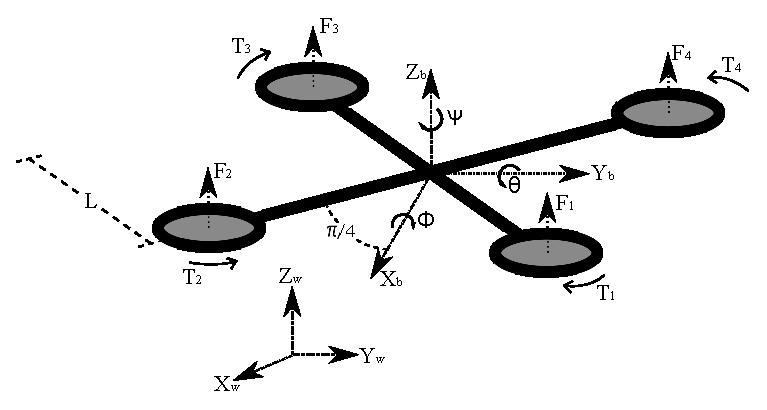
\includegraphics[width=0.97\textwidth]{quadcopter1.eps}
% figure caption is below the figure
\caption{Quadrotor geometry in `X' configuration} 
    \label{fig:quadrotorX}
    \end{center}
\end{figure}

\subsubsection{Throttle $u$ [$N$]}
\begin{equation}
u = \sum_{i=1}^{4}F_{M_i}
\end{equation}

\subsubsection{Yaw Torque $\tau_{\psi}$ [$N\cdot m$]}
\begin{equation}
\tau_{\psi} = K_{m}(F_{M_2} + F_{M_4} - F_{M_1} - F_{M_3})
\end{equation}

\subsubsection{Roll Torque $\tau_{\theta}$ [$N\cdot m$]}
\begin{equation}
\tau_{\theta} = L_{X}(F_{M_3}+F_{M_4}-F_{M_2}-F_{M_1})
\end{equation}

\subsubsection{Pitch Torque $\tau_{\phi}$ [$N\cdot m$]}
\begin{equation}
\tau_{\phi} = L_{X}(F_{M_2}+F_{M_3}-F_{M_1}-F_{M_4})
\end{equation}

\subsubsection{Inputs Setting in `X' Configuration}
$L_{X} = L\cdot \cos\left(\pi/4\right)$ is the real distance between the point of application of the rolling and pitching torques and the quadrotor center of mass along the $x$ and $y$ axes \cite{Faessler2016}.
\\\\
The rolling, pitching and yawing torques contained in vector $\tau$, are generated using the force exerted by each motor as 
\begin{equation}
	U = \begin{bmatrix}
	u\\[5pt]
	\tau_{\psi}\\[5pt]
	\tau_{\theta}\\[5pt]
	\tau_{\phi}
	\end{bmatrix} = \begin{bmatrix}
	1 & 1 & 1 & 1 \\[5pt]
	-K_{m} & K_{m} & -K_{m} & K_{m}\\[5pt]
	-L_{X} & -L_{X} & L_{X} & L_{X}\\[5pt]
	-L_{X} & L_{X} & L_{X} & -L_{X}
							\end{bmatrix}
\begin{bmatrix}
F_{M_1}\\[5pt]
F_{M_2}\\[5pt]
F_{M_3}\\[5pt]
F_{M_4}
\end{bmatrix}
	\label{ec:U_X}						
\end{equation}
where $ T_{i} $ is the torque produced by each motor along the $z_{b}$ axis, $L$ is the distance between each motor rotor and the quadrotor $CoG$, and $L_X$ is the real distance between the point of application of the rolling and pitching torques and the quadrotor $CoG$ along the $x_b$ and $y_b$ axes \cite{Faessler2016}.\\\\



\section{Nonlinear Model}
\label{sec:nonlinear}

This section describes the dynamic modeling used to perform the quadrotor control, based on the study carried out in \cite{modelamiento, modelamientoPDAFC, modelamientoNCQ}. This model represents the quadrotor as a solid symmetrical object subject to a total thrust and three torques, without considering the dynamics of the actuators.


\subsection{Euler-Lagrange Approach}
The general coordinates representing the position and attitude of the quadrotor are defined as
\begin{equation}
	q=\begin{bmatrix}
	\xi & \eta
	\end{bmatrix}^{T},
	\label{ec:coorgenerales}
\end{equation}
where $\xi=\begin{bmatrix}
x & y & z
\end{bmatrix}^{T}$ is the vector representing the position of the center of mass of the quadrotor relative to the body reference frame shown in Fig. \ref{fig:marcoreferencia} and $\eta=\begin{bmatrix}
\psi & \theta & \phi
\end{bmatrix}^{T}$ represent the quadrotor attitude.
\\\\
The Lagrangian of the quadrotor is defined by
\begin{equation}
	L(q,\dot{q})=K_{trans}+K_{rot} - U,	
	\label{ec:lagrangiano}
\end{equation}
where $ K_{trans} = \dfrac{m}{2}\dot{\xi}^{T}\dot{\xi} $ is the translational kinetic energy, $ K_{rot} = \dfrac{1}{2}\dot{\eta}^{T}J\dot{\eta} $ is the rotational kinetic energy, $ U=mgz $ is the potential energy, $m$ is the quadrotor mass , $z$ is the quadrotor elevation, $g$ is the gravity acceleration magnitude, and $J$ is the inertial matrix. The dynamic model of the quadrotor is derived from the Euler-Lagrange equation
\begin{equation}
	\dfrac{d}{dt}\dfrac{\partial L}{\partial \dot{q}}-\dfrac{\partial L}{\partial q}=
	\begin{bmatrix}
	F_{\xi}\\
	\tau
	\end{bmatrix},
	\label{ec:eulerlag}
 \end{equation} 
where $F_{\xi}=R_{b}^{w}\hat{F_{b}}$ is the translational force applied to the quadrotor by the four motors, $\tau$ contains the rolling, pitching and yawing torques, and 
\begin{equation}
R_{b}^{w} = \begin{bmatrix}
C_\theta C_\psi & C_\psi S_\theta S_\phi-C_\phi S_\psi & S_\phi S_\psi+C_\phi C_\psi S_\theta\\
C_\theta S_\psi & S_\psi S_\theta S_\phi+C_\phi C_\psi & C_\phi S_\psi S_\theta - S_\phi C_\psi\\
-S_\theta & C_\theta S_\phi & C_\theta C_\phi
\end{bmatrix}
\end{equation}
is the rotation matrix from the body to the Earth frame where $C_\theta = \cos\theta$ and $S_\theta = \sin\theta$.
\\\\
In the quadrotor body-frame, the translational force $\hat{F_{b}}$ is only applied in the $z_{b}$ axis as shown in Fig. \ref{fig:marcoreferencia}. This force is represented by
\begin{equation}
	\hat{F_{b}}=\begin{pmatrix}
	0\\
	0\\
	u
	\end{pmatrix} = \begin{pmatrix}
	0\\
	0\\
	\sum_{i=1}^{4}F_{M_i}
	\end{pmatrix}  ,
 \label{ec:fuerzas}
 \end{equation} 
with $ F_{M_i} $ being the force, in N, exerted by the motor $ M_{i}$, as shown in Fig. \ref{fig:marcoreferencia}.
\\\\
The force $ F_{M_i} $ has a linear dependency with the square of the motor angular velocity, defined as
\begin{equation}
	F_{M_i}=k_{i}w_{i}^{2},
	\label{ec:fi}
\end{equation}
where $ w_{i} $ is the angular velocity of the motor, and $ k_{i} $ is a proportional constant. However, in practice $F_{M_i}$ must be set using the PWM signal input of an ESC. The thrust-PWM relation is found experimentally and is shown in Section \ref{sec:Implementation}.
\\\\
The Euler-Lagrange equations can be divided in two parts, one for the $\xi$ coordinates and another for the $\eta$ coordinates, getting
\begin{equation}
\label{eqn:E-L1}
\ddot{\xi} =
\begin{bmatrix}
\ddot{x} \\ \ddot{y} \\ \ddot{z}
\end{bmatrix} 
=
\begin{bmatrix}
\frac{u_{1}}{m}(C_\phi S_\theta C_\psi + S_\phi S_\psi) \\
 \frac{u_{1}}{m}(C_\phi S_\theta S_\psi - S_\phi C_\psi) \\
\frac{u_{1}}{m}(C_\phi C_\theta) - g
\end{bmatrix},
\end{equation}
\begin{equation}
\label{eqn:E-L2}
\ddot{\eta} =
\begin{bmatrix}
\ddot{\psi} \\ \ddot{\theta} \\ \ddot{\phi}
\end{bmatrix} 
 =
\begin{bmatrix}
\dot{\phi}\dot{\theta}\dfrac{J_{xx}-J_{yy}}{J_{zz}} + \dfrac{u_{2}}{J_{zz}} \\
\dot{\phi}\dot{\psi}\dfrac{J_{zz}-J_{xx}}{J_{yy}} + \dfrac{u_{3}}{J_{yy}} \\
 \dot{\theta}\dot{\psi}\dfrac{J_{yy}-J_{zz}}{J_{xx}} +  \dfrac{u_{4}}{J_{xx}}
\end{bmatrix},
\end{equation}
where, $\begin{bmatrix}
u_{1},\ u_{2},\ u_{3}, \ u_{4}
\end{bmatrix}^{T} = \begin{bmatrix}
u,\ \tau_{\psi},\ \tau_{\theta},\ \tau_{\phi}
\end{bmatrix}^{T} $, and $ (J_{xx}, J_{yy}, J_{zz}) $ are the moments of inertia around the quadrotor body-frame axes \cite{Emam2016, Badr2016}.
\\\\

that is a simplified representation of the quadrotor complete model found in \cite{Bouabdallah2007}.

\subsection{Newton-Euler Approach}
sdasdasdaasd

\section{Linearized Model}
\label{sec:linearized}
\setcounter{MaxMatrixCols}{20}
\subsection{Jacobian Linearization}
\cite{Sabatino2015}
\\\\
The Euler-Lagrange equations in (\ref{eqn:E-L1}) and (\ref{eqn:E-L2}) are linearized using their Jacobian around the hover state where $\begin{bmatrix}
\eta,\ \dot{\eta},\ \dot{\xi}
\end{bmatrix} \to \begin{bmatrix}
0,\ 0,\ 0
\end{bmatrix}$, getting
\begin{equation}
\label{eqn:linear}
\ddot{q}
=
\begin{bmatrix}
g\theta \\
g\phi\\
u_{1}/m \\
u_{2}/J_{zz} \\
u_{3}/J_{yy} \\
u_{4}/J_{xx}
\end{bmatrix},
\end{equation}

As said above, in order to perform the linearization, an equilibrium point is
needed. Such an equilibrium point can be:
\begin{equation}
\overline{\mathbf{x}} = \begin{bmatrix}
\overline{x} & \overline{y} & \overline{z} & 0 & 0 & 0 & 0 & 0 & 0 & 0 & 0 & 0
\end{bmatrix}^{T}
\end{equation}
From the equations, we can find that the equilibrium point (2.29) is obtained by
the constant input value:
\begin{equation}
\overline{\mathbf{u}} = \begin{bmatrix}
mg & 0 & 0 & 0
\end{bmatrix}^{T}
\end{equation}
with $mg$ being the lift force.
\\\\
The linearized model of the quad-rotor helicopter written as a state space model is given by

\begin{align*}
\dot{\mathbf{x}}(t) = & A\mathbf{x}(t)+B\mathbf{u}(t),\\
\mathbf{y}(t) = & C\mathbf{x}(t),
\end{align*}
where
\begin{align}
\begin{split}
A  = \frac{\partial f(\mathbf{x},\mathbf{u})}{\partial \mathbf{x}}\Bigr|_{\substack{\mathbf{x}=\overline{\mathbf{x}}\\\mathbf{u}=\overline{\mathbf{u}}}} = & 
\begin{bmatrix}
0 & 1 & 0 & 0 & 0 & 0 & 0 & 0 & 0 & 0 & 0 & 0\\[2px]
0 & 0 & 0 & 0 & 0 & 0 & 0 & 0 & g & 0 & 0 & 0\\[2px]
0 & 0 & 0 & 1 & 0 & 0 & 0 & 0 & 0 & 0 & 0 & 0\\[2px]
0 & 0 & 0 & 0 & 0 & 0 & 0 & 0 & 0 & 0 & g & 0\\[2px]
0 & 0 & 0 & 0 & 0 & 1 & 0 & 0 & 0 & 0 & 0 & 0\\[2px]
0 & 0 & 0 & 0 & 0 & 0 & 0 & 0 & 0 & 0 & 0 & 0\\[2px]
0 & 0 & 0 & 0 & 0 & 0 & 0 & 1 & 0 & 0 & 0 & 0\\[2px]
0 & 0 & 0 & 0 & 0 & 0 & 0 & 0 & 0 & 0 & 0 & 0\\[2px]
0 & 0 & 0 & 0 & 0 & 0 & 0 & 0 & 0 & 1 & 0 & 0\\[2px]
0 & 0 & 0 & 0 & 0 & 0 & 0 & 0 & 0 & 0 & 0 & 0\\[2px]
0 & 0 & 0 & 0 & 0 & 0 & 0 & 0 & 0 & 0 & 0 & 1\\[2px]
0 & 0 & 0 & 0 & 0 & 0 & 0 & 0 & 0 & 0 & 0 & 0
\end{bmatrix}, \\[15px]
B = \frac{\partial f(\mathbf{x},\mathbf{u})}{\partial \mathbf{u}}\Bigr|_{\substack{\mathbf{x}=\overline{\mathbf{x}}\\\mathbf{u}=\overline{\mathbf{u}}}} = & 
\begin{bmatrix}
0 & 0 & 0 & 0 & 0 & \frac{1}{m} & 0 & 0 & 0 & 0 & 0 & 0\\[5px]
0 & 0 & 0 & 0 & 0 & 0 & 0 & \frac{1}{I_{zz}} & 0 & 0 & 0 & 0\\[5px]
0 & 0 & 0 & 0 & 0 & 0 & 0 & 0 & 0 & \frac{1}{I_{yy}} & 0 & 0\\[5px]
0 & 0 & 0 & 0 & 0 & 0 & 0 & 0 & 0 & 0 & 0 & \frac{1}{I_{xx}}
\end{bmatrix}^{T},\\[15px]
C = &
\begin{bmatrix}
1 & 0 & 0 & 0 & 0 & 0 & 0 & 0 & 0 & 0 & 0 & 0\\
0 & 0 & 1 & 0 & 0 & 0 & 0 & 0 & 0 & 0 & 0 & 0\\
0 & 0 & 0 & 0 & 1 & 0 & 0 & 0 & 0 & 0 & 0 & 0\\
0 & 0 & 0 & 0 & 0 & 0 & 1 & 0 & 0 & 0 & 0 & 0 
\end{bmatrix},
\end{split}
\end{align}

with the parameters  

$m=0.64 $ kg, 

$g=9.81$ m/s.


The state vector is defined as

\begin{align*}
x(t)=&
\begin{bmatrix}
r_x & \dot{r}_x & r_y & \dot{r}_y & r &\dot{r}_z 
\end{bmatrix}^T,
\end{align*}
and the control inputs as
\begin{align*}
u(t)=&
\begin{bmatrix}
u_1 & u_2 &u_3 & u_4
\end{bmatrix}^T,
\end{align*}

and the output vector is defined as

\begin{align*}
r(t)=
\begin{bmatrix}
r_{x} & r_{y} & r_{z}
\end{bmatrix}^T.
\end{align*}

\subsection{Thrust Compensation}
\url{https://robotics.stackexchange.com/questions/4247/tilt-compensated-motor-output-to-keep-altitude-for-quadcopter}
Recalling the rotation matrix $R_{b}^{w}$,
\begin{equation}
R_{b}^{w} = \begin{bmatrix}
c\theta c\psi & c\psi s\theta s\phi-c\phi s\psi & s\phi s\psi+c\phi c\psi s\theta\\
c\theta s\psi & s\psi s\theta s\phi+c\phi c\psi & c\phi s\psi s\theta - s\phi c\psi\\
-s\theta & c\theta s\phi & c\theta c\phi
\end{bmatrix}
\end{equation}
\begin{equation}
u = u^{*} \cos{\theta}\cos{\phi}
\end{equation}
\begin{equation}
u^{*} = \dfrac{u}{\cos{\theta}\cos{\phi}}
\end{equation}
\section{Conclusions}
This chapter presented the design of the two vehicles developed in this thesis.
The test-bench and the OS4. The first system is only capable of 3 DoF which
facilitates the testing of the controllers. However, it is possible to detach the
flying part in order to test free flights. Before designing the second system
which is a free flying quadrotor, a new design methodology is introduced. It
allows an optimal design of small-scale rotorcraft. Four new design indicators
were introduced for a precise and complete evaluation of the design performance.
This methodology appreciably facilitated the components selection
process and battery dimensioning of OS4. This quadrotor exhibits higher
capabilities and endurance than the competition. This is verified through
the comparison of different design parameters. OS4 embeds all the necessary
avionics and energy devices for a fully autonomous flight. This comprises a
low cost IMU, a vision based position sensor specifically developed for this
project and an obstacle detection setup.

